\section{Module 2: Lecture 3\\Signals and Vectors}

%\subsection{Introduction}
%In the previous lecture, we have learnt how a periodic input given to a Linear Shift Invariant system results in a periodic output with the same period. Now in this lecture we will see some new concepts by which every input can be expressed as sinusoidal inputs. Henceforth, it will be simpler to analyse their outputs.

\subsection{Relations between Signals and Vectors}
Consider a 2-dimensional vector. We can decompose this vector into two perpendicular components with $e_1$ and $e_2$ as the unit vectors along those directions. To find these components, we need to use the dot product.
\subsubsection{Dot Product}
	The dot product of two vectors $u$ and $v$ is defined as the magnitude of the vector $u$ multiplied by the magnitude of the vector $v$ multiplied by the cosine of the angle between these two vectors.
    \begin{equation*}u.v = |u||v|cos\theta\end{equation*}
  where $\theta$ is the angle between the vectors $u$ and $v$. If $u$ is a unit vector, then the dot product of vectors $v$ and $u$ gives the component of the vector $v$ in the direction of $u$, with the value $|v|\cos \theta$.
	\begin{figure}[ht]\label{fig:vector-decomposition}
    \centering
    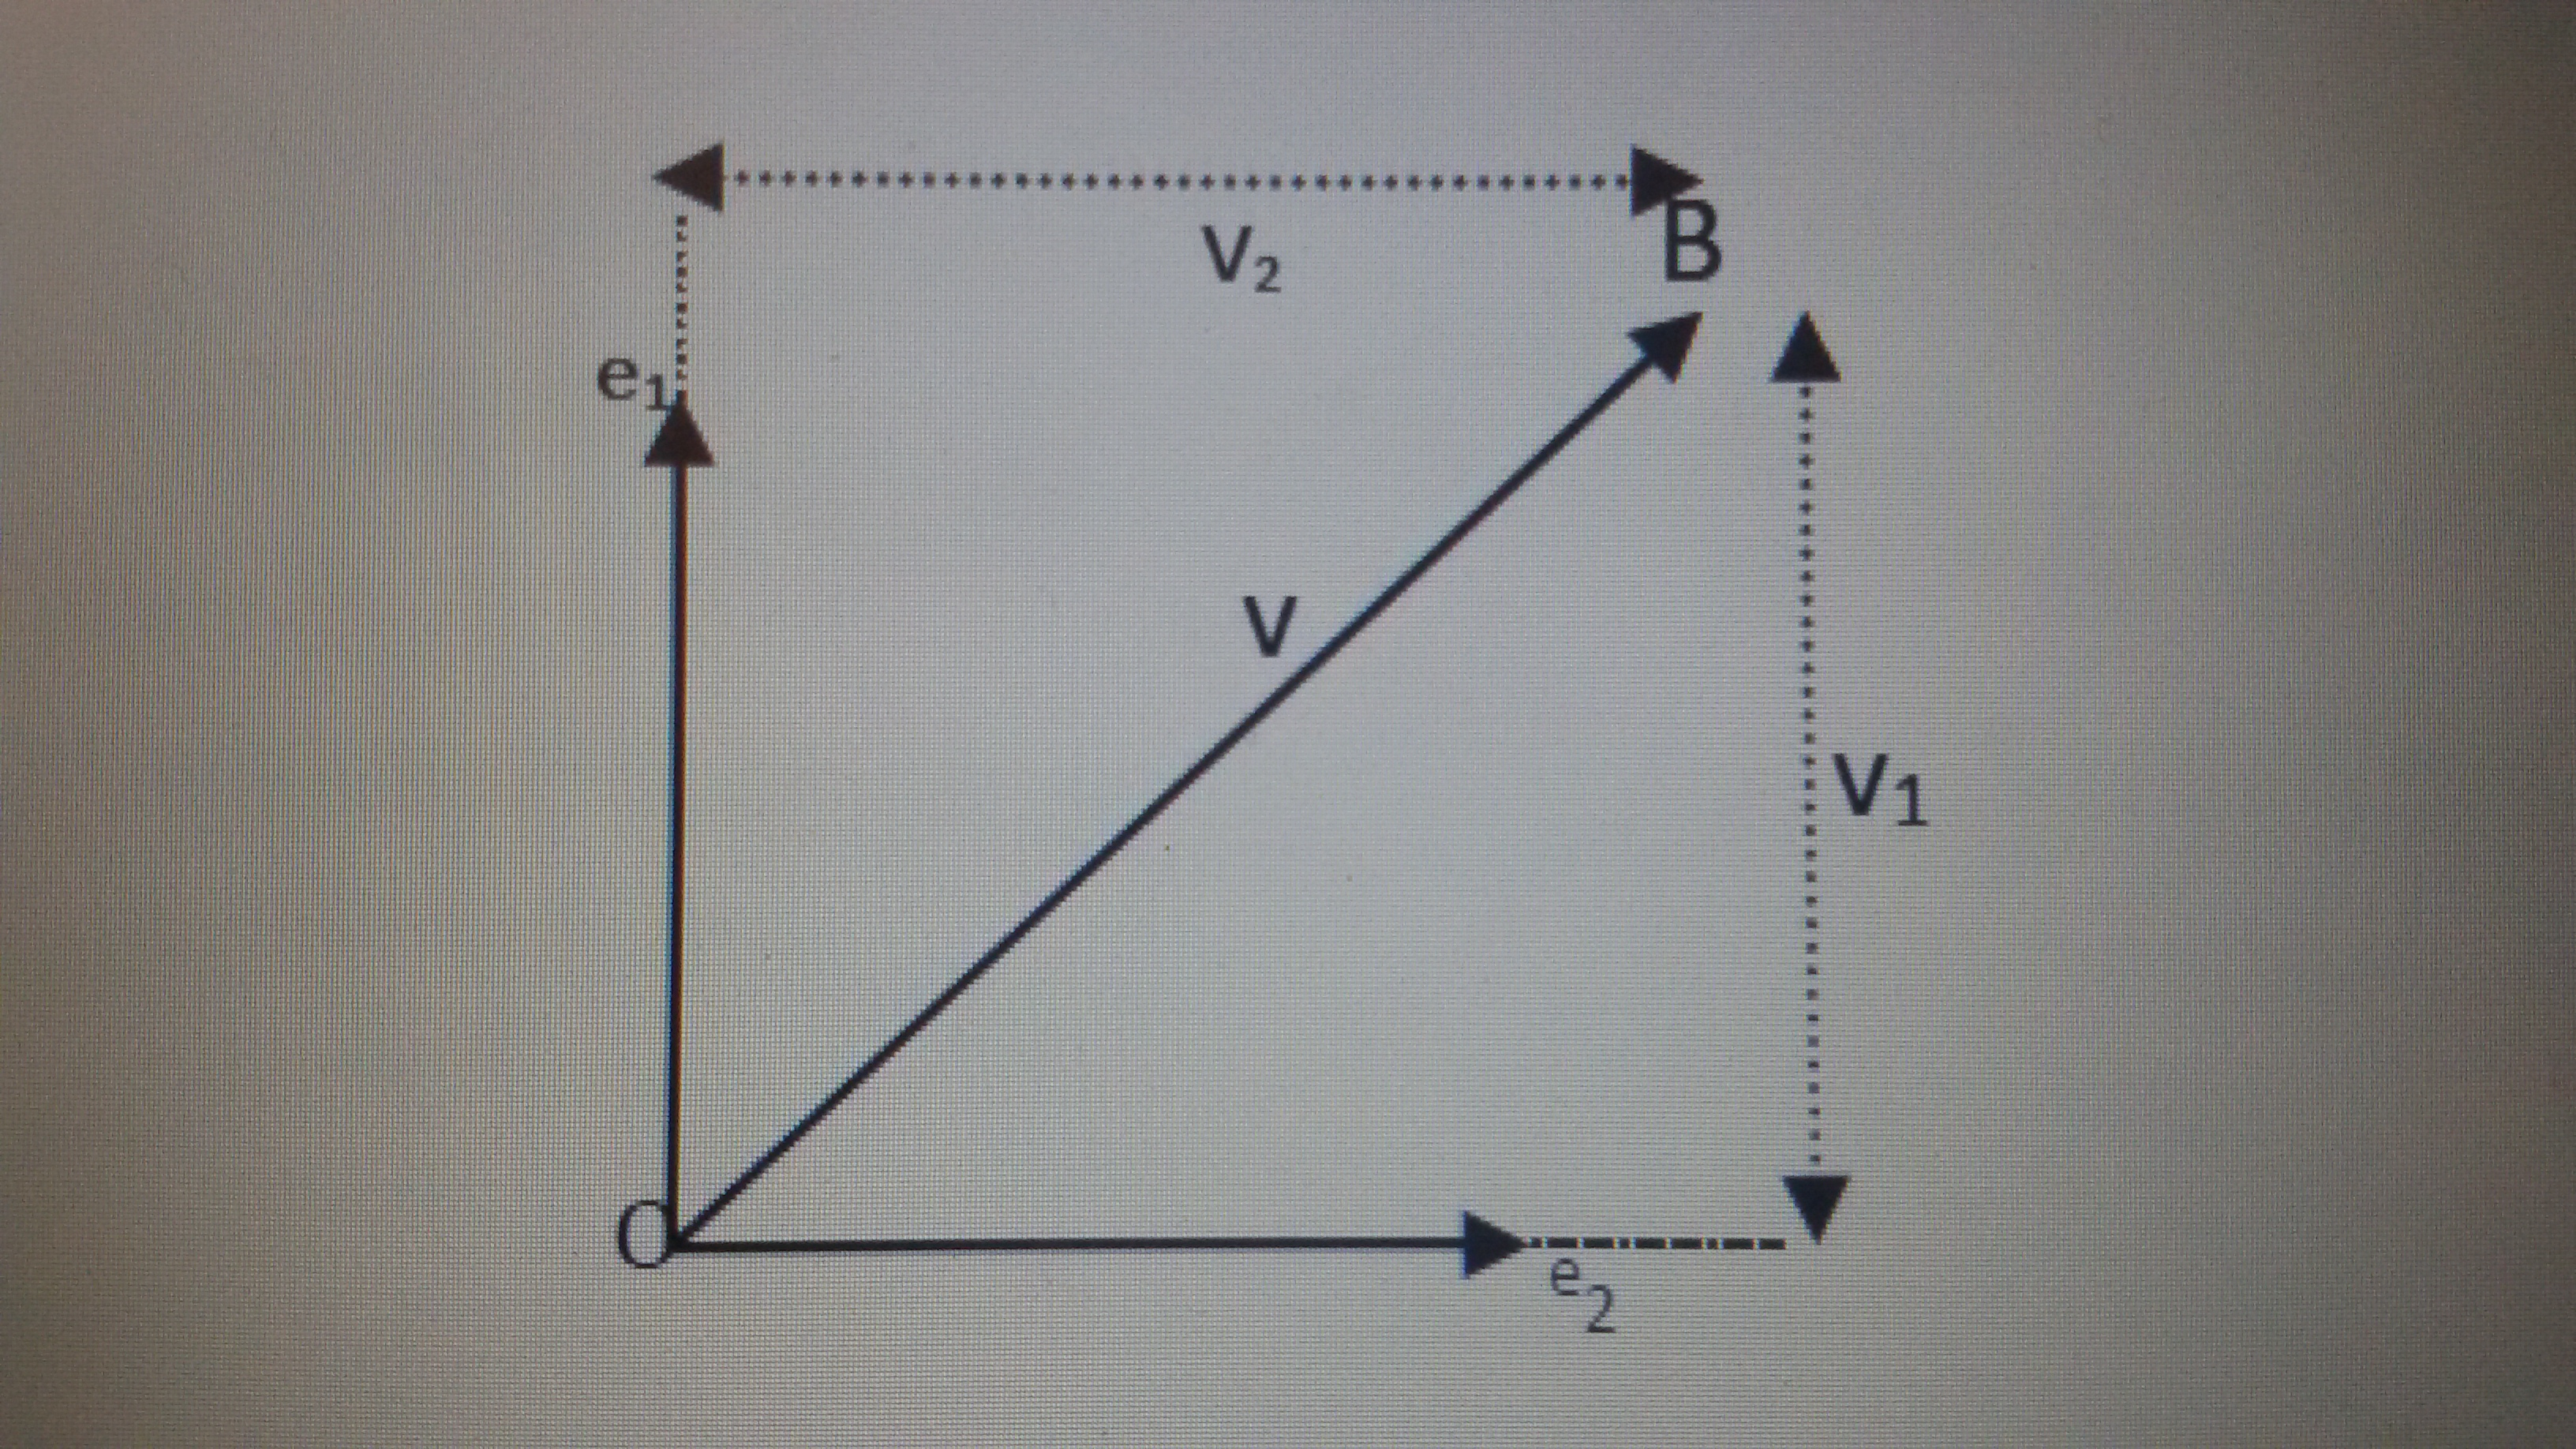
\includegraphics[scale=0.08]{figure.jpg}
  \end{figure} 
  In Fig.\ref{fig:vector-decomposition}, OB is a vector denoted by $v$ which is expressed as
    \begin{equation*}v = v_1e_1 + v_2e_2\end{equation*}
    
    where $v_1$ and $v_2$ are the components in the $e_1$ and $e_2$ directions respectively. In this way, we can express any vector as a linear combination of $e_1$ and $e_2$. Thus, we can say that the vectors $e_1$ and $e_2$ span the 2D space.
    % A collection of vectors span a space.
    Suppose if any vector can be expressed uniquely as a linear combination of $\{ u_1$,$u_2$,$u_3$ .... $u_n \}$, where $\{ u_1$,$u_2$,$u_3$...$u_n \}$ are linearly independent, then $\{ u_1$,$u_2$...$u_n \}$ is said to form a basis.\\
\noindent
Also, if $\langle u_i$,$u_j \rangle$ = 0 for $i,j \in [1,n]$ and $i \neq j$, i.e. the dot product of any two distinct basis vectors is zero,  then the basis is said to be an \emph{orthogonal basis}. Finally, for a $n-$dimensional space, a collection of $n$ linearly independent vectors forms the basis.\\
\noindent
The dot product of two vectors $u$ and $v$ is equal to the sum of the products of the corresponding perpendicular components. Suppose

				\begin{equation*}u = u_1e_1 + u_2e_2\end{equation*}
                        
                        \begin{equation*}v = v_1e_1 + v_2e_2\end{equation*} 
\noindent                        
                        then,\begin{equation*} u.v = u_1v_1 + u_2v_2\end{equation*}
           
\subsubsection{Dot Product of Discrete Sequences}           
Now, consider a discrete sequence with $2$ non-zero points. This sequence can be compared to a $2-$dimensional vector $v$ with $v_1$ and $v_2$ as its perpendicular components such that it is equal to the values at the $2$ non-zero points of the sequence. Similarly for a sequence with $n$ non-zero points can be considered as a vector in $n-$dimensional space. Also, the concept of dot product is similarly applied to the discrete sequences.\\
For example, consider
\begin{equation*}
  x[n] = (1/2)^n u[n]
\end{equation*}
    i.e.
\begin{align*}
  x[n] &= (1/2)^n	\ \text{for} \ n\geq0 \\
  &= 0 \ \text{for} \ n<0
\end{align*}

\begin{equation*}
  y[n] = (1/3)^nu[n]
\end{equation*}
i.e. 
\begin{align*}
  y[n] &= (1/3)^n \ \text{for} \ n\geq0 \\
  &= 0 \ \text{for} \ n<0
\end{align*}
                  
                  
  Let's calculate the dot product of $x[n]$ and $y[n]$, i.e. sum the product of the corresponding components.
  We have,
   \begin{equation*} \langle x[n],y[n] \rangle = \sum_{n=-\infty}^{\infty}\ x[n]y[n]\end{equation*} 
   \begin{equation*} \langle x[n],y[n] \rangle = \sum_{n=0}^{\infty}\ x[n]y[n]\end{equation*} 
   \begin{equation*} \langle x[n],y[n] \rangle = \sum_{n=0}^{\infty}\ (1/2)^n*(1/3)^n\end{equation*} 
   \begin{equation*} \langle x[n],y[n] \rangle = \sum_{n=0}^{\infty}\ (1/6)^n\end{equation*} 
   \begin{equation*} \langle x[n],y[n] \rangle = \frac{1}{(1-(1/6))}\end{equation*} 
   \begin{equation*} \langle x[n],y[n] \rangle = \frac{6}{5}\end{equation*} 
  		
          
 	This is the dot product of the two discrete sequences. This dot product is also called as the \emph{inner product}. The inner product of two vectors $u$ and $v$ is represented by $\langle u,v \rangle$.

\subsubsection{Inner Product of Continuous Signals}
       In a discrete sequence, a unit vector can be expressed as $\delta[n-N]$ for all $N \in \mathbb{Z}$. An $n-$dimensional vector $v$ can be expressed as
        \begin{equation*}v = v_1e_1 + v_2e_2 + ........ + v_ne_n\end{equation*}
        Now writing the above equation in terms of sequences, we have
       
    	\begin{equation*}	x[n] = 	\sum_{N=-\infty}^{\infty}\ x[N]\delta[n-N]\end{equation*}
            
            where $x[N]$ is the component along the dimension $N$.
       
Applying the same concept for continuous time functions, we need to replace the summation by an integral, which gives,

					\begin{equation*}x(t) = \int_{-\infty}^{\infty} \! x(\lambda)\delta[t-\lambda] \ \mathrm{d}\lambda\end{equation*}
                    
             where $x(\lambda)$ is the component in the direction $\lambda$ and $\delta[t-\lambda]$ is continuous impulse at $\lambda$ similar to a unit vector. So, the inner product of $x(t)$ and $y(t)$ is given by
             
           \begin{equation*} \langle x(t),y(t) \rangle = \int_{-\infty}^{\infty} \! x(t)y(t) \ \mathrm{d} t\end{equation*}
             
 \subsection{Sinusoids as basis vectors}
          Let us see how we can express any periodic signal as a linear combination of sinusoids. We first need to find sinusoidal signals which are perpendicular. Consider a signal $x(t)$ which is periodic with period $T$,i.e. 
          \begin{equation*}
            x(t) = x(t+T) \ \forall \ t 
          \end{equation*}
          Assume that it can be expressed as a sum of sinusoidal functions. We should take a sinusoidal function which is periodic with period $T$. So it is of the form $A_k\cos (\frac{2\pi}{T}kt + \phi_k)$. We have,
          
          \begin{equation*}x(t) = \sum_{k=-\infty}^{\infty}\ A_k\cos (\frac{2\pi}{T}kt + \phi_k)\end{equation*}
          Let's take two different $k$'s.
\begin{equation*}
x_1 (t) = A_1 \cos (\frac{2\pi}{T}k_1t + \phi_1)
\end{equation*}
           and \begin{equation*}
x_2 (t) = A_2 \cos (\frac{2\pi}{T}k_2t + \phi_2)
\end{equation*}
          Consider the inner product of $x_1(t)$ and $x_2(t)$ with the interval going from $0$ to $T$. We are here restricting our interval to $T$ because the integral might diverge when we integrate from $0$ to $\infty$. We have,
           \begin{equation*}\langle x_1(t),x_2(t) \rangle = \int_{0}^{T} \! x_1(t)x_2(t) \ \mathrm{d}t\end{equation*}
           \begin{equation*}\langle x_1 (t),x_2 (t) \rangle = \int_{0}^{T} \! \cos (\frac{2\pi}{T}k_1t + \phi_1) \cos (\frac{2\pi}{T}k_2t + \phi_2) \ \mathrm{d}t\end{equation*}
           Using 
          \begin{equation*} 2\cos A \cos B = \cos(\frac{A+B}{2}) + \cos(\frac{A-B}{2})\end{equation*}
          We have,
          \begin{equation*}\langle x_1 (t),x_2 (t) \rangle = \int_{0}^{T} \! \frac{1}{2} \left\lbrace \cos (\frac{2\pi}{T}\frac{(k_1+k_2)}{2}t + \frac{\phi_1+\phi_2}{2}) + \cos (\frac{2\pi}{T}\frac{(k_1-k_2)}{2}t + \frac{\phi_1-\phi_2}{2}) \right\rbrace \ \mathrm{d}t \end{equation*}
                If ($k_1$ + $k_2$) or ($k_1$ - $k_2$) are not zero, that means we have a finite number of cycles of the sinusoids, implying the integral is zero. However if $k_1$=$k_2$, the second integral becomes $T/2$ times $\cos ((\phi_1-\phi_2)/2)$.
                Thus we have,
            \begin{equation*} \langle x_1 (t),x_2 (t) \rangle  \neq 0	\enspace \enspace	\text{for} \enspace k_1 = k_2\end{equation*}
            \begin{equation*} \langle x_1 (t),x_2 (t) \rangle = 0	\enspace \enspace		\text{for} \enspace k_1 \neq k_2\end{equation*}
                Hence, we have proved that two sinusoids with the same time period are perpendicular if they don't have the same angular frequency and vice-versa. Using this important concept, we will be able to write any periodic signal as sum of sinusoidal signals and hence analysis of these signals will be simpler.

